\section{État des lieux}

\subsection{Principes à respecter pour un affichage élégant}

%\begin{frame}
%	\frametitle{Principes à respecter pour un affichage élégant}
%	\textit{Idée : dessiner un arbre élégant et montrer ce qui le rend élégant. Entourer les noeuds au même niveau pour le principe 2, etc etc. Mais ne pas cumuler. Faire une pseudo-animation pour montrer un principe à chaque étape de l'animation, l'un après l'autre}
%	\begin{enumerate}
%		\item Les arêtes de l'arbre ne doivent pas s'intersecter.
%		\item Les n\oe{}uds de même profondeur doivent être dessinés sur la même ligne horizontale.
%		\item Les arbres doivent être dessinés de la manière la plus compacte possible.
%		\item Un n\oe{}ud parent doit être centré par rapport à ses fils.
%		\item Un sous-arbre doit être dessiné de la même façon, peu importe où il est placé dans l'arbre.
%		\item Les n\oe{}uds fils d'un n\oe{}ud père doivent être espacés de manière homogène.
%	\end{enumerate}
%\end{frame}

\begin{frame}
	\begin{center}	
		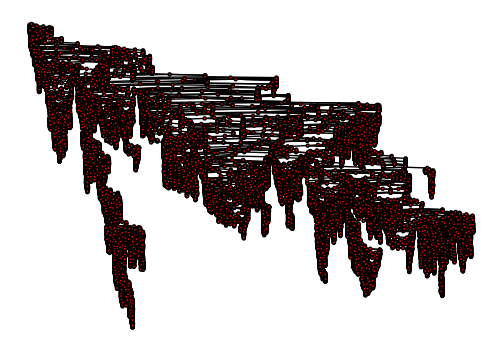
\includegraphics[width=7cm]{exempleIntro}<1->\\
		\begin{block}{Principe 1}<2->
		Les arêtes de l'arbre ne doivent pas s'intersecter.
		\end{block}
	\end{center}
\end{frame}

\begin{frame}
	\begin{center}	
		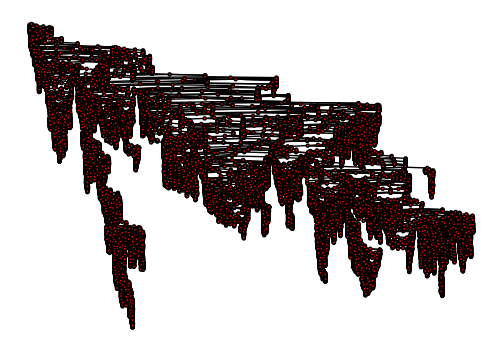
\includegraphics[width=7cm]{exempleIntro}<1->\\
		\begin{block}{Principe 2}<2->
		Les n\oe{}uds de même profondeur doivent être dessinés sur la même ligne horizontale.
		\end{block}
	\end{center}
\end{frame}

\begin{frame}
	\begin{center}	
		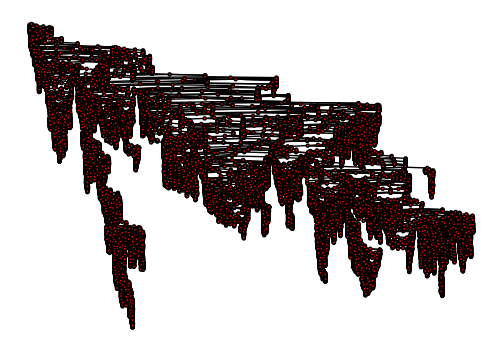
\includegraphics[width=7cm]{exempleIntro}<1->\\
		\begin{block}{Principe 3}<2->
		Les arbres doivent être dessinés de la manière la plus compacte possible.
		\end{block}
	\end{center}
\end{frame}

\begin{frame}
	\begin{center}	
		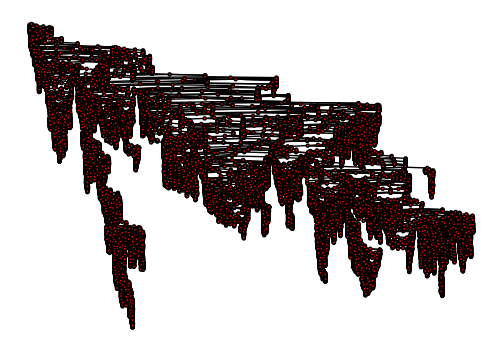
\includegraphics[width=7cm]{exempleIntro}<1->\\
		\begin{block}{Principe 4}<2->
		Un n\oe{}ud parent doit être centré par rapport à ses fils.
		\end{block}
	\end{center}
\end{frame}

\begin{frame}
	\begin{center}	
		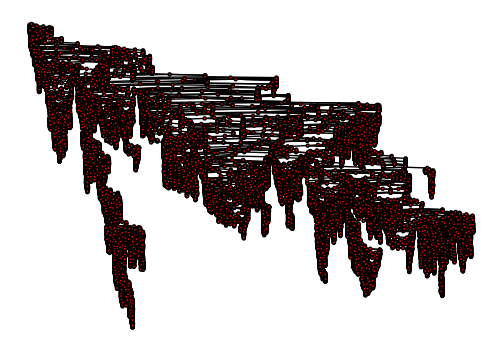
\includegraphics[width=7cm]{exempleIntro}<1->\\
		\begin{block}{Principe 5}<2->
		Un sous-arbre doit être dessiné de la même façon, peu importe où il est placé dans l'arbre.
		\end{block}
	\end{center}
\end{frame}

\begin{frame}
	\begin{center}	
		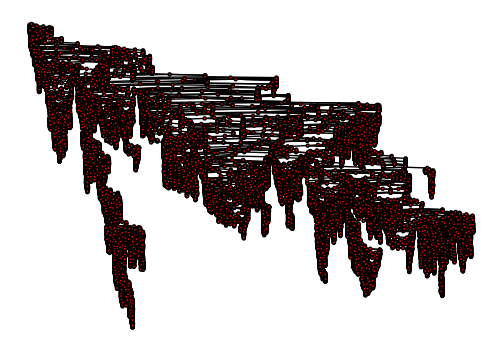
\includegraphics[width=7cm]{exempleIntro}<1->\\
		\begin{block}{Principe 6}<2->
		Les n\oe{}uds fils d'un n\oe{}ud père doivent être espacés de manière homogène.
		\end{block}
	\end{center}
\end{frame}

\subsection{Algorithmes existants}

\begin{frame}
	\frametitle{Knuth}
	\begin{center}
	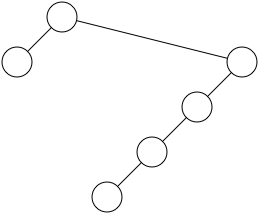
\includegraphics[height=3.5cm]{knuth}
	\end{center}
	Décrit une idée de "slot disponible"\\
	Inconvénient :
	\begin{itemize}
		\item Ne respecte que les principes 1 et 2
	\end{itemize}
\end{frame}

\begin{frame}
	\frametitle{Algorithmes de Charles Wetherell et Alfred Shannon}
	\begin{center}
	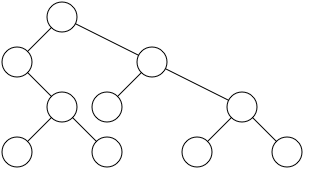
\includegraphics[height=3.5cm]{shannon}
	\end{center}
	Approche Bottom Up pour centrer le père sur ses fils\\
	Introduction d'un tableau de slots\\
	Inconvénient :
	\begin{itemize}
		\item Ne respecte pas les principes 4 et 5
	\end{itemize}
\end{frame}

\begin{frame}
	\frametitle{The Mods and the Rockers}
	Traitement en deux passes\\
	Avantage :
	\begin{itemize}
		\item Respecte tous les principes
	\end{itemize}
	Inconvénient
	\begin{itemize}
		\item Ne concerne que les arbres binaires
	\end{itemize}
\end{frame}

%\chapter{État des lieux}
%
%\paragraph{}Les articles que nous avons étudiés concernaient avant tout la visualisation des arbres binaires de grande taille sans prendre en compte l'ordre des fils. Il en ressort néanmoins plusieurs principes :
%\begin{enumerate}
%	\item Les arêtes de l'arbre ne doivent pas s'intersecter.
%	\item Les n\oe{}uds de même profondeur doivent être dessinés sur la même ligne horizontale.
%	\item Les arbres doivent être dessinés de la manière la plus compacte possible.
%	\item Un n\oe{}ud parent doit être centré par rapport à ses fils.
%	\item Un sous-arbre doit être dessiné de la même façon, peu importe où il est placé dans l'arbre.
%	\item Les n\oe{}uds fils d'un n\oe{}ud père doivent être espacés de manière homogène.
%\end{enumerate}
%
%\paragraph{}Un des enjeux soulevés par l'ensemble de ces principes est que les n\oe{}uds ne doivent pas se chevaucher, tout comme les arbres en eux-même.
%
%\paragraph{}Il existe plusieurs algorithmes permettant de dessiner des arbres de grande taille, mais tous ne respectent pas tous les principes décrits ci-dessus.
%
%\subparagraph{}Par exemple, l'algorithme le plus simple, l'algorithme de Knuth \cite{REF_Knuth}, ne respecte que les deux premiers principes. Cet algorithme décrit déjà une idée de "slot disponible". Mais ce sont Charles Wetherell et Alfred Shannon \cite{REF_Wetherell}, en 1979, qui introduiront l'utilisation d'un tableau qui associera à chaque profondeur le prochain slot disponible. Ils arrivent ainsi à respecter tous les principes, à l'exception des principes 4 et 5. Ils introduisent malgré tout également l'idée de parcourir l'arbre de bas en haut, plutôt que l'inverse, ceci afin de centrer facilement un père selon ses fils.
%
%\subparagraph{}Le principal problème est alors : Comment respecter tous ces principes et traiter le chevauchement d'arbres sans perdre en complexité ? C'est l'algorithme The Mods and the Rockers qui répondra à cette question. Au lieu de reparcourir les sous-arbres pour les décaler afin d'éviter tout chevauchement, on raisonne en deux passes de l'arbre. Lors de la première passe, on mémorise un \emph{modifier} qui indiquera le décallage qui devra être appliqué sur chaque sous-arbre lors de la deuxième passe.
%
%\subparagraph{}Il existe enfin des algorithmes dont le but est surtout d'optimiser les concepts et algorithmes existants. Citons le concept de contour d'arbre, qui permet de ne parcourir que ce contour et donc de ne pas rentrer au c\oe{}ur de l'arbre. Ceci est un gain conséquent puisque nous traitons ici des arbres de grande taille, et donc potentiellement très larges.
%
%\paragraph{}Nous allons donc voir à présent comment nous nous sommes inspirées de ces algorithmes afin de généraliser les concepts aux arbres n-aires, et en conservant l'ordre des fils.